\section{Arbeitsmarkt}
Arbeitslosigkeit existiert dann, wenn Haushalte bereit sind zum Marktlohn Arbeit anzubieten, diee aber nicht vom Unternehmen nachgefragt werden.\\
Keine Arbeitslosigkeit herrscht dann, wenn Haushalte den Marktlohn als zu tief empfinden und deshalb keine Arbeit anbieten.\\
Zwei Typen der Arbeitslosigkeit\\
\begin{minipage}{10cm}
	\begin{itemize}
		\item \textbf{Sockelarbeitslosigkeit (X)}
		\item Anzahl der offenen Stellen ist gleich oder grösser als die Anzahl der Arbeitslosen (strukturelle und friktionelle Arbeitslosigkeit)
		\item \textbf{Konjukturelle Arbeitslosigkeit (Y)}
		\item Anzahl der Arbeitslosen ist grösser als Anzahl der offenen Stellen
	\end{itemize}
\end{minipage}
\begin{minipage}{5cm}
	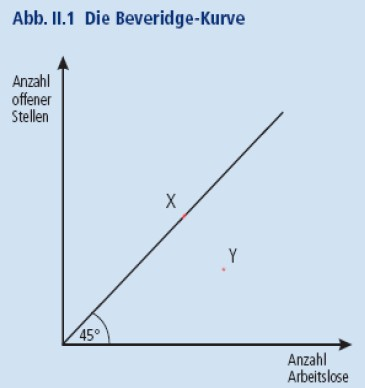
\includegraphics[width=5cm]{images/beveridge.jpg}
\end{minipage}
\subsection{Messung der Arbeitslosigkeit}
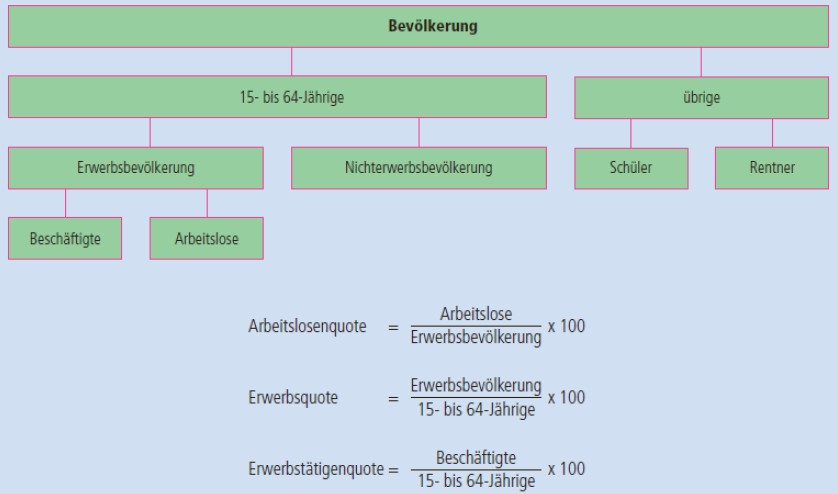
\includegraphics[width=0.8\linewidth]{images/messung.jpg}
\subsection{Der flexible Arbeitsmarkt}
\begin{multicols}{2}
	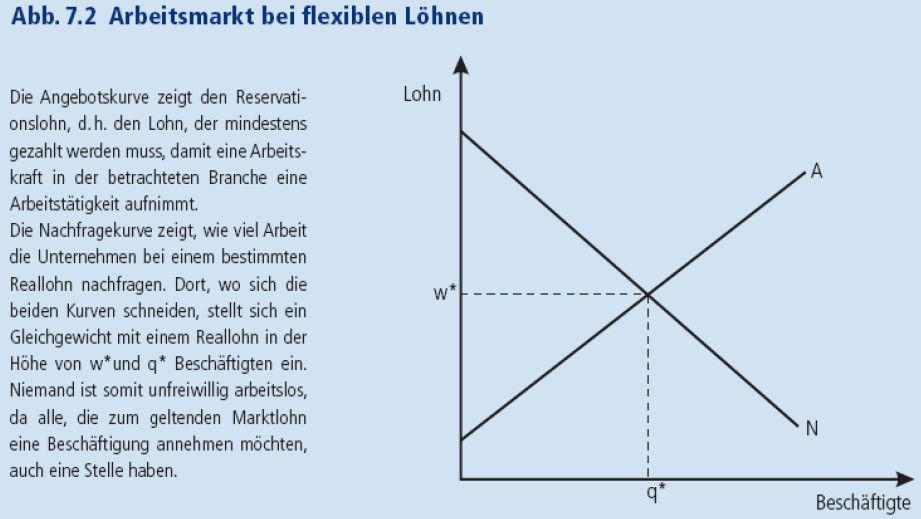
\includegraphics[width=0.5\linewidth]{images/flexibellohne.jpg}
	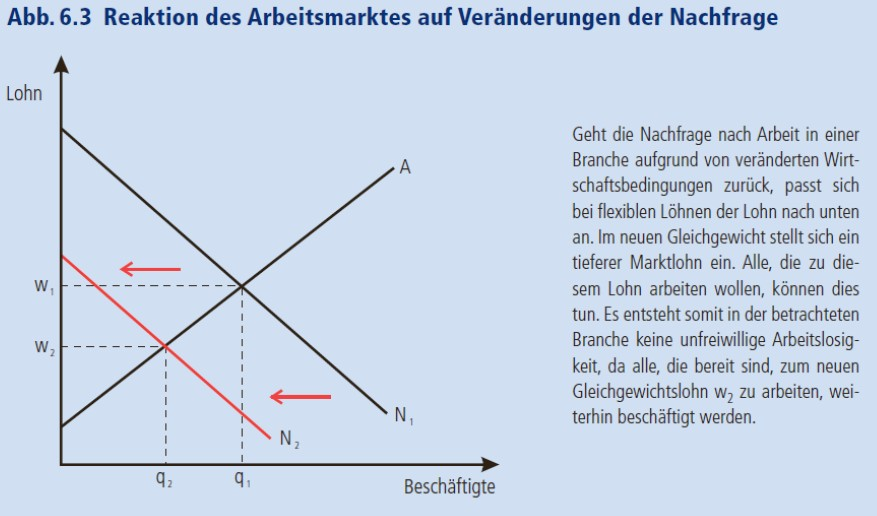
\includegraphics[width=0.5\linewidth]{images/flexibellohne2.jpg}
\end{multicols}
\subsection{Der regulierte Arbeitsmarkt}
	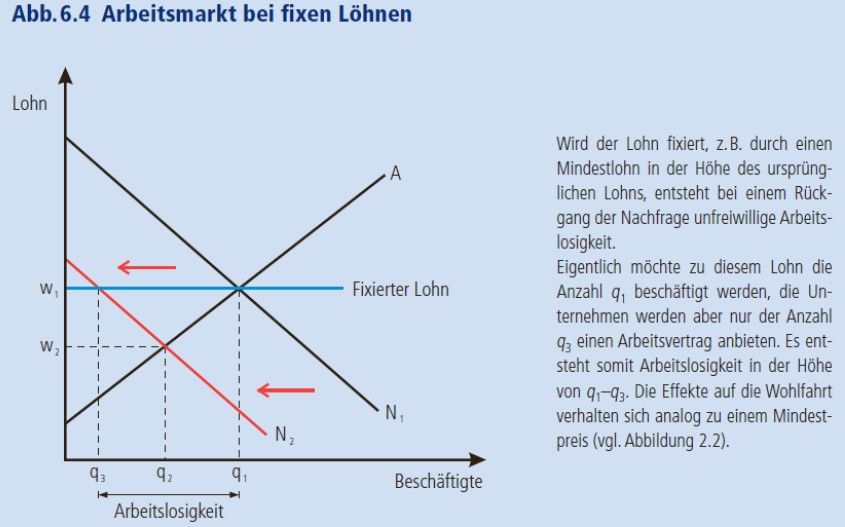
\includegraphics[width=0.8\linewidth]{images/fixelohne.jpg}
\subsection{Sockelarbeitslosigkeit}
\begin{itemize}
	\item \textbf{Strukturelle}
	\subitem Mindestlöhne
	\subitem Zentralisierte Lohnverhandlungen
	\item \textbf{Friktionelle}
	\subitem Ausgestaltung Arbeitslosigkeit
	\subitem Zeitspanne zum Finden einer neuen Stelle
\end{itemize}
\subsection{Arbeitsmarktpolitik der Schweiz}
\begin{enumerate}
	\item Mindestlöhne
	\subitem CH: Keine branchenübergreifende Mindestlöhne
	\item Zentralisierte Lohnverhandlungen
	\subitem CH: nur dezentral auf Branchenebene
	\item Regulierungen bezüglich Anstellungen und Entlassunge
	\subitem CH: wenig
	\item Ausgestaltung der Arbeitslosenversicherung
	\subitem CH: setzt auf Wiedereingliederung
	\item Regulierung der Arbeitszeit
	\subitem CH: wenig
\end{enumerate}